% 学位论文 : 第一章  绪论
% 
% 更新记录:
%   {$LastChangedBy$}
%   {$LastChangedRevision$}
%   {$LastChangedDate$}

\chapter{绪论}

\section{研究背景}


随着社会的发展与科学技术的进步,人们对信息服务的需求量与日俱增,信息产业已经成为关系国计民生的支柱性产业。世界各国纷纷投入大量的资金、人力、物力,致力于发展本国的信息产业,美国“信息高速公路”,韩国“IT大运河”,欧盟“宽带战略”等等,信息产业已经成为体现一个国家综合国力的重要指标。为了适应全球信息产业革命的进程,《国家中长期科学和技术发展规划纲要》明确提出:到2020 年,我国要“掌握一批事关国家竞争力的装备制造业和信息产业核心技术,使制造业和信息产业技术水平进入世界先进行列。”作为现代信息技术的主要载体,光传输网络的发展在我国信息产业建设中起着举足轻重的作用。所以,光网络的发展就成为我国信息产业建设的首要任务。同时,这种战略上的重大需求也给人们带来了各种技术上的挑战。如何建设功能更强、可靠性更好,功耗及成本更低、体积更小、使用维护更方便的光通信网络,成为信息技术研究人员所关注的热点。

显然,为了实现以上研究目标,单纯地依靠网络层面的优化是远远不够的,基础器件层面的进展更能够带动光通信网络的重大发展。目前,光通信器件还大多是相互独立,依靠传统的技术手段将其连接,组合成光网络。为了进一步降低成本,减小器件体积,光电子集成(即光电子器件之间,光电子与微电子器件之间的集成)就成为光通信器件的大势所趋。我们知道,制备光电子器件(如激光器,探测器,放大器等等)的基本材料都是半导体材料,尤其是Ⅲ-Ⅴ族半导体材料,为了实现不同器件之间的集成,不同的半导体材料之间的异质兼容就成为一个重要的研究方向。目前,光电子器件主要是GaAs基与InP基器件,微电子器件则是以Si基为主,而且,Si基造价低廉,应用广泛,且对于1.3-1.6μm的通信波长范围,Si是透明的,所以, Si基与GaAs基器件的异质兼容,一方面对光电子集成具有重大意义,另一方面能够有效地降低器件的制作成本。

自1963年阿尔费洛夫和克罗默两位科学家提出了半导体双异质结构以来,光电子器件经过了将近半个世纪的发展,已经取得了丰硕的成果,为光通信产业的快速发展起到了不可替代的推动作用。然而,相对于目前已经发展成熟的Si基大规模集成电路而言,光电子器件的集成度还不可同日而语。因此,将Si与III-V族材料集成成为了长期以来一个重要的研究方向。


\section{技术难点}

在本研究中,我们关注的是GaAs在Si衬底上的异质外延。两者的材料属性如下表所示

\begin{table*}[htbp] 
	\centering
	\caption{\label{tab:TimeXDR}不同生长时间XDR测试结果}  
	\begin{tabular}{m{.2\textwidth}<{\centering}m{.2\textwidth}<{\centering}m{.2\textwidth}<{\centering}m{.2\textwidth}<{\centering}}  
		\toprule
			半导体材料 & 晶格结构 & 晶格常数 & 热膨胀系数(300K) \\
		\midrule 
			Si & 金刚石结构 & 5.430 & 2.6×10-6 \\
			GaAs & 闪锌矿结构 & 5.653 & 6.8×10-6 \\
		\bottomrule
	\end{tabular}
\end{table*}

从该表可以看出,Si与GaAs之间在晶格结构、晶格常数和热膨胀系数之间有很大的不同。

{\hei 晶格常数的不同}

在室温下,Si的晶格常数要比GaAs小4.1\%,这就意味着当在Si衬底上外延GaAs时,GaAs为了与下面的Si衬底的原子相匹配,每沉积25行原子,就要清除一个Ga或As原子的平面。然而,没有其他的III-V族半导体合金材料与Si的晶格失配要小于GaAs与Si的晶格失配。在图\ref{fig:LatticeConstant}中画出了常见的半导体材料晶格常数与带隙能之间的关系。可以看出,GaAs是和Si最匹配的直接带隙二元化合物半导体材料。

\begin{figure}[ht]
	\centering
	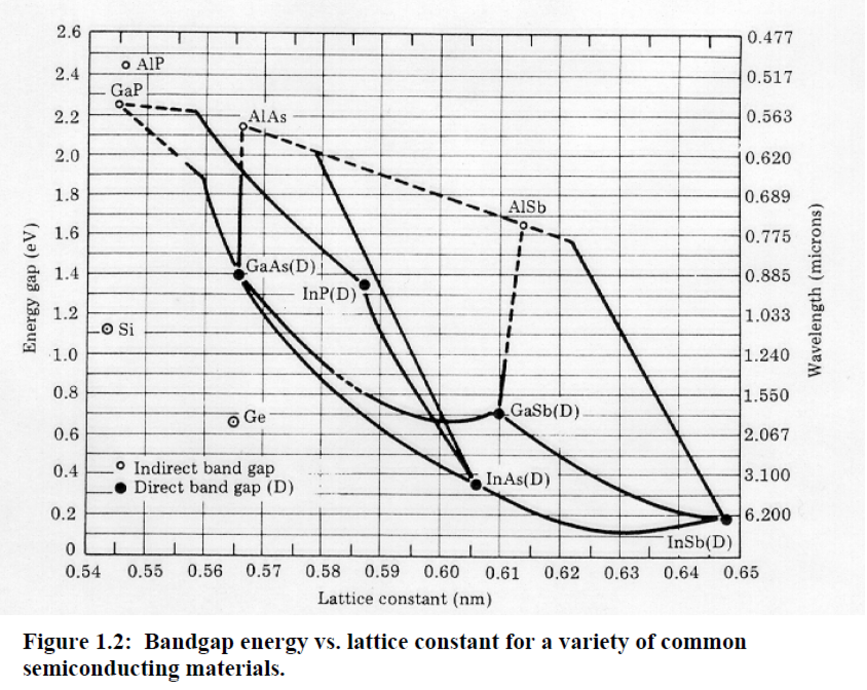
\includegraphics[width=0.8\textwidth]{ch01_LatticeConstant.pdf}
	\caption{常见的半导体材料晶格常数与带隙能之间的关系}
	\label{fig:LatticeConstant}
\end{figure}

对于Si基的III-V族外延,如果晶格失配是不可避免的,则考虑到这个失配怎样影响半导体晶体生长的过程是很重要的。当晶格常数为af的半导体沉积到晶格常数为as的衬底上,则两者所产生的失配应变就可以定义为:

\begin{equation}
	\label{eq:f}
	f = \frac{a_s-a_f}{a_f}
\end{equation}

如果失配较小,则失配应变则会转变为沉积薄膜的弹性形变。如果外延薄膜晶格常数大于衬底晶格常数则是压应变,反之,则是张应变。在每一种情况下,衬底与外延薄膜都保持着连贯性,即衬底的每一个原子都与唯一的外延薄膜原子成键。对于失配较大或外延薄膜较厚的材料,当界面处的失配应变超过相干半导体原子之间成键弹性能,失配应变就会增加。在这个临界点处,薄膜就会产生弹性形变,导致原子键断裂和衬底-薄膜界面非相干晶体位错的形成。图\ref{fig:ElasticStrain}是压应变的半导体薄膜沉积到衬底上的赝形生长和异变生长的截面示意图。

\begin{figure}[ht]
	\centering
	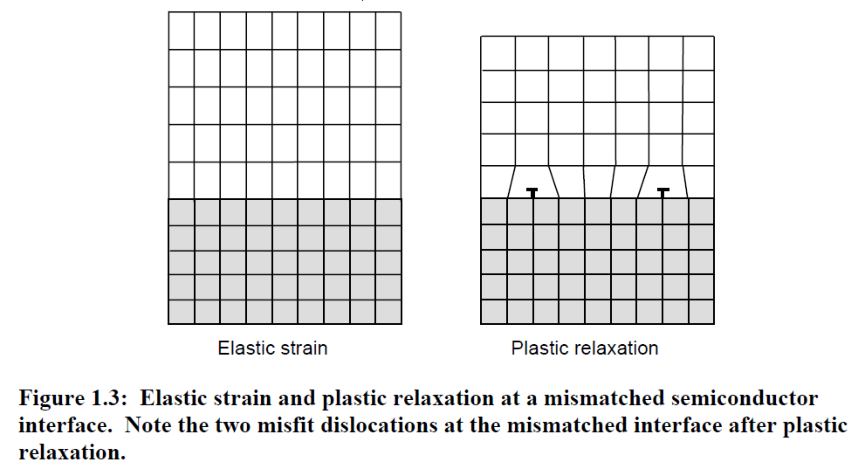
\includegraphics[width=0.8\textwidth]{ch01_ElasticStrain.pdf}
	\caption{压应变的半导体薄膜沉积到衬底上的赝形生长和异变生长的截面示意图}
	\label{fig:ElasticStrain}
\end{figure}

从图中可以看出,为了释放失配应变,半导体薄膜会在衬底-薄膜界面会产生一维线破坏原子键。这个一维的位错结构就是失配位错,失配位错会沿着界面线性滑移,并终止于晶体的自由表面。对于经常用于半导体器件外延的(001)表面,失配晶体的{111}<110>滑移系统会使失配位错线沿着能量较低的[110]和[11 ̅0]方向调整自己。一旦形成,位错线可以就通过位错沿失配界面的滑移增长。

所有的失配位错都会在半导体晶片的自由表面界面终止。在金刚石结构或闪锌矿结构材料中,位于衬底和外延薄膜处的失配位错线通过穿透位错与表面连接,位错沿{111}平面的应变失配界面向上穿透。在半导体材料中穿透位错是一维的晶体位错,并不会释放应变。在异质外延集成的光电子器件中,穿透位错是非辐射复合中心,严重影响了器件的发光性能,因此减少穿透位错的产生是异质外延生长中一项重要的工作。

在失配半导体薄膜中,当薄膜的厚度超过平衡临界厚度时,在界面处会以多种方式形成失配和穿透位错。当失配应变很大时,失配位错环通过同质成核形成,但是在实际的生长系统里,这个机制很少发生,而更常见的是在缺陷表面或者是点位错的地方位错环异质成核。失配位错也可以在穿透位错从衬底向上攀移的过程中形成。图\ref{fig:DislocationNucleation}是在失配系统中位错形成的不同方式的原理图。

\begin{figure}[ht]
	\centering
	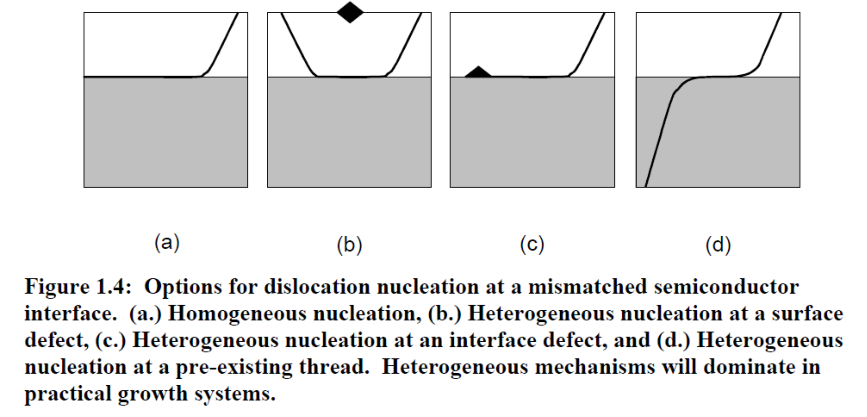
\includegraphics[width=0.8\textwidth]{ch01_DislocationNucleation.pdf}
	\caption{失配系统中位错形成的不同方式的原理图}
	\label{fig:DislocationNucleation}
\end{figure}

要想在给定的应变条件下成功的进行应变层异质外延生长,就要降低穿透位错密度。在上面也提到过,在光电子器件中穿透位错是非辐射复合中心,这是因为在位错芯局部的中间带隙能级对注入的少数载流子的复活效率很高。对少数载流子的俘获使得材料中少数载流子的寿命大幅减少。少数载流子寿命的减少对于半导体激光器是不利的。对于半导体激光器,只有在有源层实现大量的少数载流子反转才能得到有效的增益效率并产生激光。在激光器结构中,如果由于位错使得少数载流子寿命减少,更多注入的少数载流子在达到足够的粒子数反转的数量之前会形成非辐射重组。早期的研究工作指出,对于GaAs基的激光器,当穿透位错密度超过$106cm^{-2}$时,由于受到少数载流子寿命减少的影响,激光器不能正常工作。对于现在的GaAs基激光器已经不存在这个问题(现在的商用GaAs衬底穿透位错密度已经达到$100cm^{-2}$),然而对于现在的Si基外延的GaAs薄膜,穿透位错密度接近$109cm^{-2}$,这就是在Si衬底上集成GaAs基激光器的主要问题。

{\hei 热膨胀系数不同}


\section{研究现状}
我来占个位置。\cite{BUPT_Thesis_Format_2004}


% 本章参考文献
\ifx\usechapbib\empty
\bibliographystyle{buptthesis}
\bibliography{bare_thesis}
\fi

%%% Local Variables: 
%%% mode: latex
%%% TeX-master: "bare_thesis"
%%% End: 
